% ==============================================================================
% LATEX TIKZ / PGFPLOTS SNIPPET: K-FAC ENGAGEMENT & RHO MEAN DYNAMICS OVER EPOCHS
% ==============================================================================
% This snippet plots the dynamic allocation of Second-Order (K-FAC) preconditioning
% AND the Curvature Anisotropy Ratio (rho_mean) across the 200 training epochs,
% reading directly from CSVs_ablation/trinity_kfac_dynamics.csv.
%
% Requirements in Preamble:
%   \usepackage{tikz}
%   \usepackage{pgfplots}
%   \usepackage{pgfplotstable}
%   \usepackage{subcaption}
%   \pgfplotsset{compat=1.18}
% ==============================================================================

% Color definitions (compatible with paper theme)
\definecolor{colorwrn}{RGB}{31, 119, 180}     % Steel Blue (Wide-ResNet-101-2)
\definecolor{colorvit}{RGB}{148, 103, 189}    % Purple (Vision Transformer)
\definecolor{colorresnet}{RGB}{44, 160, 44}   % Forest Green (ResNet-18)
\definecolor{colorthresh}{RGB}{120, 120, 120} % Neutral Gray for threshold

% ==============================================================================
% OPTION 1: PGFPLOTS TIKZ (PERFECT COLUMN WIDTH USAGE, ZERO DEAD SPACE)
% ==============================================================================
\begin{figure}[!t]
  \centering
  \resizebox{\columnwidth}{!}{%
  \begin{tikzpicture}
    % --- AXIS 1 (LEFT): K-FAC ALLOCATION (%) ---
    \begin{axis}[
      name=ax1,
      width=3.6cm,
      height=2.9cm,
      scale only axis,
      xmin=1, xmax=200,
      ymin=-1, ymax=46,
      xtick={1,100,200},
      ytick={0,10,20,30,40},
      xlabel={Epoch},
      ylabel={K-FAC Blocks (\%)},
      xlabel style={font=\footnotesize, yshift=2pt},
      ylabel style={font=\footnotesize, xshift=1pt},
      tick label style={font=\scriptsize},
      title={\textbf{(a) K-FAC Allocation (\%)}},
      title style={font=\small, yshift=-2pt},
      grid=both,
      minor grid style={line width=0.2pt, draw=black!5},
      major grid style={line width=0.35pt, draw=black!12, dashed},
      legend style={
        at={(1.12, 1.26)},
        anchor=south,
        font=\fontsize{5.2}{6.2}\selectfont,
        fill=white,
        fill opacity=0.95,
        draw=black!25,
        rounded corners=1pt,
        legend columns=2,
        /tikz/every even column/.append style={column sep=0.15cm}
      }
    ]
      % Budget Cap Reference Lines
      \addplot[line width=0.5pt, color=colorwrn, dotted, domain=1:200, forget plot] {38.10};
      \addplot[line width=0.5pt, color=colorresnet, dotted, domain=1:200, forget plot] {28.57};
      \addplot[line width=0.5pt, color=colorvit, dotted, domain=1:200, forget plot] {21.05};

      % Solid Curves: K-FAC %
      \addplot[line width=1.4pt, color=colorwrn, mark=none] 
        table [x=epoch, y=wrn_so_pct, col sep=comma] {CSVs_ablation/trinity_kfac_dynamics.csv};
      \addlegendentry{Wide-ResNet-101-2 (Cap: $38.1\%$, 40/105 blks)}

      \addplot[line width=1.4pt, color=colorresnet, mark=none] 
        table [x=epoch, y=res_so_pct, col sep=comma] {CSVs_ablation/trinity_kfac_dynamics.csv};
      \addlegendentry{ResNet-18 (Cap: $28.6\%$, 6/21 blks)}

      \addplot[line width=1.4pt, color=colorvit, mark=none] 
        table [x=epoch, y=vit_so_pct, col sep=comma] {CSVs_ablation/trinity_kfac_dynamics.csv};
      \addlegendentry{Vision Transformer (Cap: $21.1\%$, 8/38 blks)}
    \end{axis}

    % --- AXIS 2 (RIGHT): CURVATURE ANISOTROPY RHO ---
    % Anchored directly to ax1.north east with exact clearance for y-labels
    \begin{axis}[
      name=ax2,
      at={(ax1.north east)},
      anchor=north west,
      xshift=0.88cm,
      width=3.6cm,
      height=2.9cm,
      scale only axis,
      xmin=1, xmax=200,
      ymin=-0.02, ymax=1.05,
      xtick={1,100,200},
      ytick={0.0,0.2,0.4,0.6,0.8,1.0},
      xlabel={Epoch},
      ylabel={Anisotropy Ratio $\bar{\rho}$},
      xlabel style={font=\footnotesize, yshift=2pt},
      ylabel style={font=\footnotesize, xshift=1pt},
      tick label style={font=\scriptsize},
      title={\textbf{(b) Curvature Ratio $\bar{\rho}$}},
      title style={font=\small, yshift=-2pt},
      grid=both,
      minor grid style={line width=0.2pt, draw=black!5},
      major grid style={line width=0.35pt, draw=black!12, dashed}
    ]
      % Curves: rho mean
      \addplot[line width=1.4pt, color=colorwrn, mark=none] 
        table [x=epoch, y=wrn_rho, col sep=comma] {CSVs_ablation/trinity_kfac_dynamics.csv};

      \addplot[line width=1.4pt, color=colorresnet, mark=none] 
        table [x=epoch, y=res_rho, col sep=comma] {CSVs_ablation/trinity_kfac_dynamics.csv};

      \addplot[line width=1.4pt, color=colorvit, mark=none] 
        table [x=epoch, y=vit_rho, col sep=comma] {CSVs_ablation/trinity_kfac_dynamics.csv};
    \end{axis}
  \end{tikzpicture}%
  }
  \caption{\textbf{Dynamic K-FAC Preconditioning Engagement and Curvature Anisotropy Evolution.} (a) Fraction of parameter blocks allocated to second-order K-FAC updates across training epochs, bounded by user budget caps (dotted lines: $38.1\%$ for WRN, $28.6\%$ for ResNet-18, $21.1\%$ for ViT). (b) Evolution of the mean curvature anisotropy ratio $\bar{\rho}$ tracked by the zeroth-order sensor as optimization progresses.}
  \label{fig:kfac_engagement_and_rho}
\end{figure}


% ==============================================================================
% OPTION 2: PRE-RENDERED VECTOR PDF (ZERO TIKZ OVERHEAD, EXACT COLUMNWIDTH)
% ==============================================================================
% If you prefer instant compilation without PGFPlots memory overhead:
% \begin{figure}[!t]
%   \centering
%   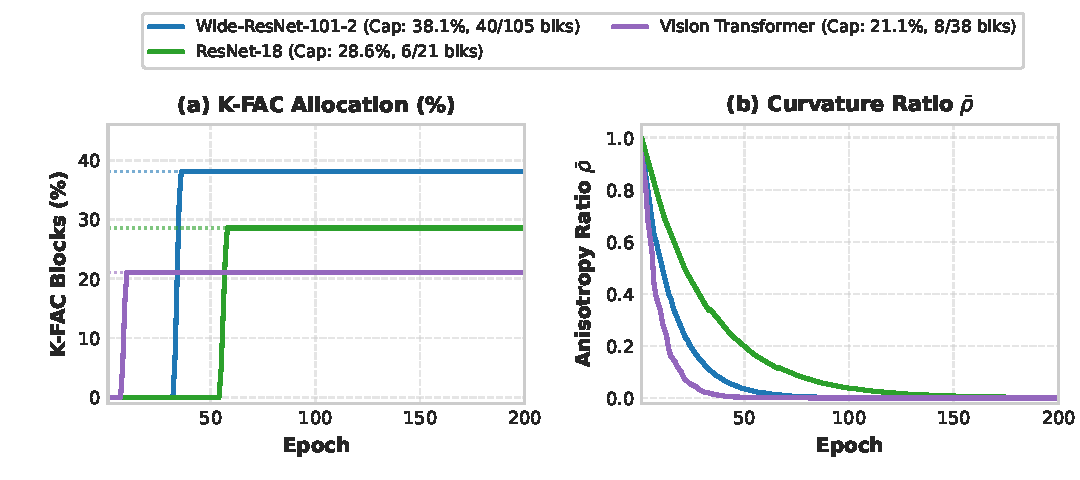
\includegraphics[width=\columnwidth]{figs/kfac_dynamics_1col_2panel.pdf}
%   \caption{\textbf{Dynamic K-FAC Allocation and Curvature Anisotropy Evolution.} (a) Fraction of parameter blocks allocated to second-order K-FAC updates across training epochs, bounded by user budget caps (dotted lines). (b) Evolution of the mean curvature anisotropy ratio $\bar{\rho}$ tracked by the zeroth-order sensor.}
%   \label{fig:kfac_engagement_and_rho}
% \end{figure}
